\section{Radio Frequency Identification}
%https://en.wikipedia.org/wiki/Near-field_communication

Its predecessor originally being a Russian invention, identification via electromagnetic waves fist saw the light of day in 1945 in the form of an espionage tool. \cite{2008hacking} This was called "The Thing" and was a bugging device used by the Russians to spy on its enemies during the start of the cold war. \cite{tvedt_2018} When activated through exterior radio waves it  would pick up sound waves through a diaphragm changing the shape of the resonator, which in turn modulated the frequency of the reflected signal. This is where the "The Thing" comes in as the forebear to RFID. as it would only work when energized by a radio carrier wave provided externally.\\

The first time Radio Frequency Identification (RFID) was implemented in its modern form was in an invention patented on January 23, 1973 by Mario Cardullo. \cite{cardullo1973transponder} This was a basic radio transponder with memory, essentially what an RFID tag is today. It had 16 bits of memory and was intended for use in toll roads to make large multiple lane toll roads, like showed in figure \ref{fig:tollroad}, obsolete. 
\begin{figure}[H]
    \centering
    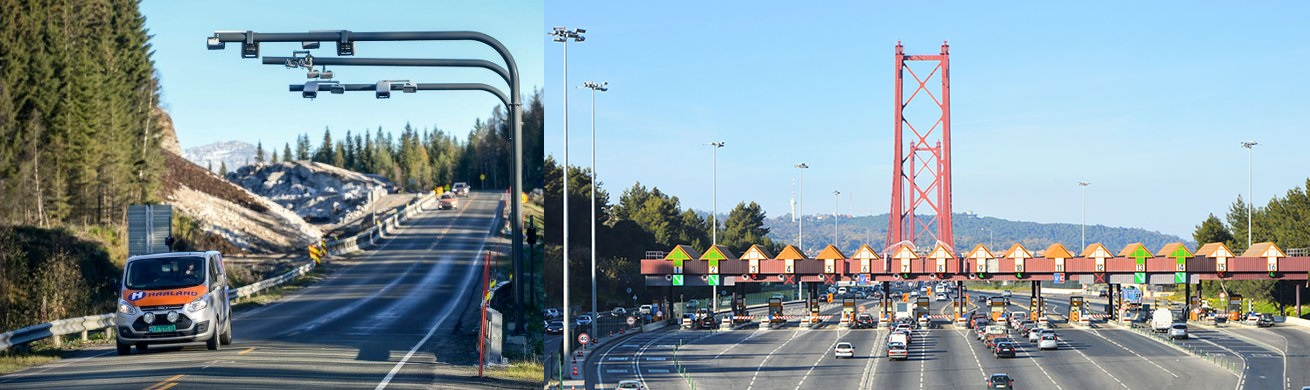
\includegraphics[width=\textwidth]{02_Literature_study/figures/vegpakke-1.jpg}
    \caption{Automatic toll road on the left and a manual at the right}
    \label{fig:tollroad}
\end{figure}

The advantage of this is both environmental and a convenience for the drivers.

\subsection{Tags}
Tags come in many shapes and sizes. The most wide-spread once in our daily life are stickers, key-chain and credit card size. Common for all is that they hold some information that can identify it. In terms of networking, they can be viewed as the "client" side in the system. \cite{cardullo2005genesis}\\

A tag can be read-only where a factory will assign the ID to the tag, or re-writable where a user can redefine the data in the data-field multiple times . A read-only tag is what one would use for systems where the ID is to be stored in a database, such as for building access. On the other hand, re-writable tags are preferable when a user would like to encode data into the tag at will.\\

An example might be a store that wants to switch from bar-codes to RFID. It would then be necessary to be able to write the same ID to all products of the same kind.


\subsubsection{Passive}
Passive tags are defined by their absence of an internal power source. Because of this feature, they are very easy and cheap to manufacture, thereby becoming the most widely used form of tag in today's RFID systems. They achieve this by harvesting their power from the electromagnetic field set up by the reader. This approach will impede the solutions effective range. A near-field electromagnetic field set up by a coil antenna will diminish by $\frac{1}{r^3}$. This is called a magnetic dipole antenna. \cite{antennadesign}

\subsubsection{Active}

Active tags are defined as a tag that has an internal power source. Therefore the tag can actively broadcast its ID without necessarily being asked for it. This is often used where long-range communication is preferable. As such, they are often used at much higher frequencies, typically in the hundreds of megahertz, as true antennas become feasible to produce, and thus enabling long-range communication. The internal power source makes them a good choice in areas with high levels of RF interference. \cite{2008hacking}
\newpage
\subsection{Reading distance}

The range of a reading device is mostly determined by the frequency, antenna effect, and the use of passive versus active tags. \cite{dipankar2009rfid, weis2007rfid} Antenna effect is in most countries regulated to avoid unnecessarily high interference. Since frequency has a large role to play, RFID is implemented on several bands to accomodate different needs.

\begin{table}[H]
\caption{Range and usecases for some of the RFID bands}
\begin{tabular}{llll}
\hline
Frequency range  & Range    & Some use-cases & Cost (Alibaba.com)\\
\hline
120-150 kHz (LF) & 1-10cm   & Building access, Animal id                & 0.02\$ <\\
13.56MHz (HF)    & 1-100cm  & Vicinity cards,  NFC                      & 0.01\$ <\\
433 MHz (UHF)    & 1-100m   & Smart home, Defence                       & 0.01\$ <\\
865-868 MHz      & 1-12m    & EAN, Railrodes                            & 0.05\$ <\\
\hline
\end{tabular}
\label{tab:RFIDranges}
\end{table}

From table \ref{tab:RFIDranges} we see that in an application aimed at detecting chess pieces on a chessboard using either the 13.56MHz or the 125kHz band would be the way to go. 

\subsubsection{Reader and tag size}
A design guide made by Microchip Technology Inc. \cite{microID125} states that the reading distance correlates to the size of the antenna coil and the tag in the following manner

\begin{table}[H]
\centering
\caption{Reading distance with regard to physical size of tag and antenna coil}
\label{my-label}
\begin{tabular}{c|cccc}
\hline
\diagbox[width=10em]{Antenna size}{Tag size}    & 1,3 cm    & 2,5 cm    & 5 cm  & 5 x 9 cm \\\hline
7,5 x 15 cm & 4 cm      & 10 cm     & 15 cm & 17,5 cm \\
50 x 140 cm & 23 cm     & 53 cm     & 76 cm & 100 cm \\
\hline
\end{tabular}
\end{table}

\newpage
\subsection{Use-cases}
RFID has a wide array of use-cases, so wide in fact that trying to list them all would be a difficult task. However here are some of the more well known uses:
\begin{itemize}
    \item RFID cards
    \begin{itemize}[\FilledSmallSquare]
        \item Cashless \cite{cashless2018}
        \item Library cards
        \item Access card
        \item Tickets
        \item Seasonal sport passes (football/skiing)
        \item Public transport
        \end{itemize}
    \item Passport
    \item Animal identification
    \item Human implants
    \item Inventory systems
    \item Postal service
    \item Toll roads
    \item Anti-theft systems
    \item Employeeless stores
\end{itemize}

\newpage
\subsubsection{Norsk Lastbærer Pool}
In 2011 a Norwegian company called \textit{Norsk Lastbærer Pool} (NLP) added RFID tags to their plastic  pallets. \cite{swedberg2011norsk} They used a form of Ultra High Frequency (UHF) RFID called EPC Gen 2. \cite{roberti2004epcglobal} NLP provide the necessary infrastructure needed to register the pallets. This gives the possibility for registering goods, both when the truck leaves the distributor, and when it arrives at the customer. As can be seen in figure \ref{fig:02:NLP} the registration is done by a portal which contains a reader, much like an industrial scale version of the portal found at the entrances of many stores.
\begin{figure}[H]
    \centering
    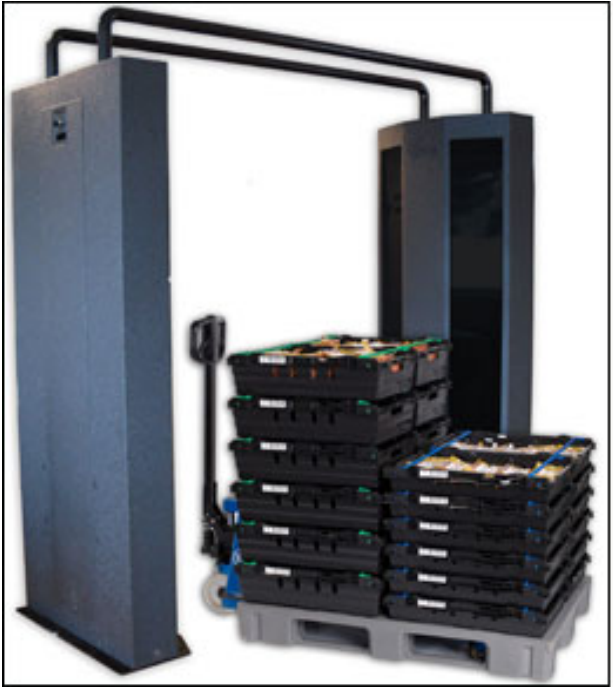
\includegraphics[width=0.5\textwidth]{02_Literature_study/figures/NLP.png}
    \caption{An illustration of the NLP pallet registration system. \cite{swedberg2011norsk}}
    \label{fig:02:NLP}
\end{figure}


\subsubsection{Amazon Go}
Amazon Go, a pilot project for employeeless convenient stores. On January 22nd, 2018 it opened to the public. \cite{bosa_salinas_2018} It has been speculated to use RFID in some part of their solution based on a patent filed in 2014. \cite{AmazonGo} The patent ways to detect items being picked up, in conjunction with computer vision it can register which customer picked it up. They do in fact have such confidence in their solution, that if you happen to walk out with a product that did not get registered, its free. \cite{bosa_salinas_2018} 

\newpage
\section{Current RFID solutions}

Microchip has published several RFID reference design already, but they are not what you would call a minimal BOM solution. One such reference design can be found in appendix \ref{appendix:ASKreader}. This solution has 74 components, and the circuit board it compiles to is in the region of 10 x 5 cm. For a chessboard application with squares that are from 4 x 4 cm to 6x6 cm. Moreover 20 years old, and the modern MCUs are more capable, being more noise tolerant and having more accurate peripherals.\\


Back in 2012, a German engineer by the name of Vassilis Serasidis designed an RFID reader circuit using the ATtiny13 \cite{attiny13} MCU and later for the ATtiny85 \cite{attiny85} in 2014. From figure \ref{fig:02:ATtiny13Circuit} it is apparent that in terms of BOM size, this approach has more potential than the one from 1998.

\begin{figure}[H]
    \centering
    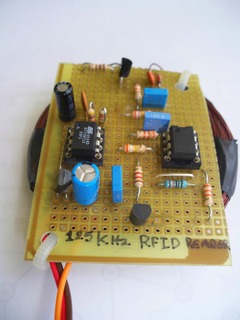
\includegraphics[width=0.5\textwidth]{02_Literature_study/figures/RFID_ATtiny13.jpg}
    \caption{Vassilis Serasidis RFID reader circuit}
    \label{fig:02:ATtiny13Physical}
\end{figure}

\begin{landscape}
 \begin{figure}
  \centering
  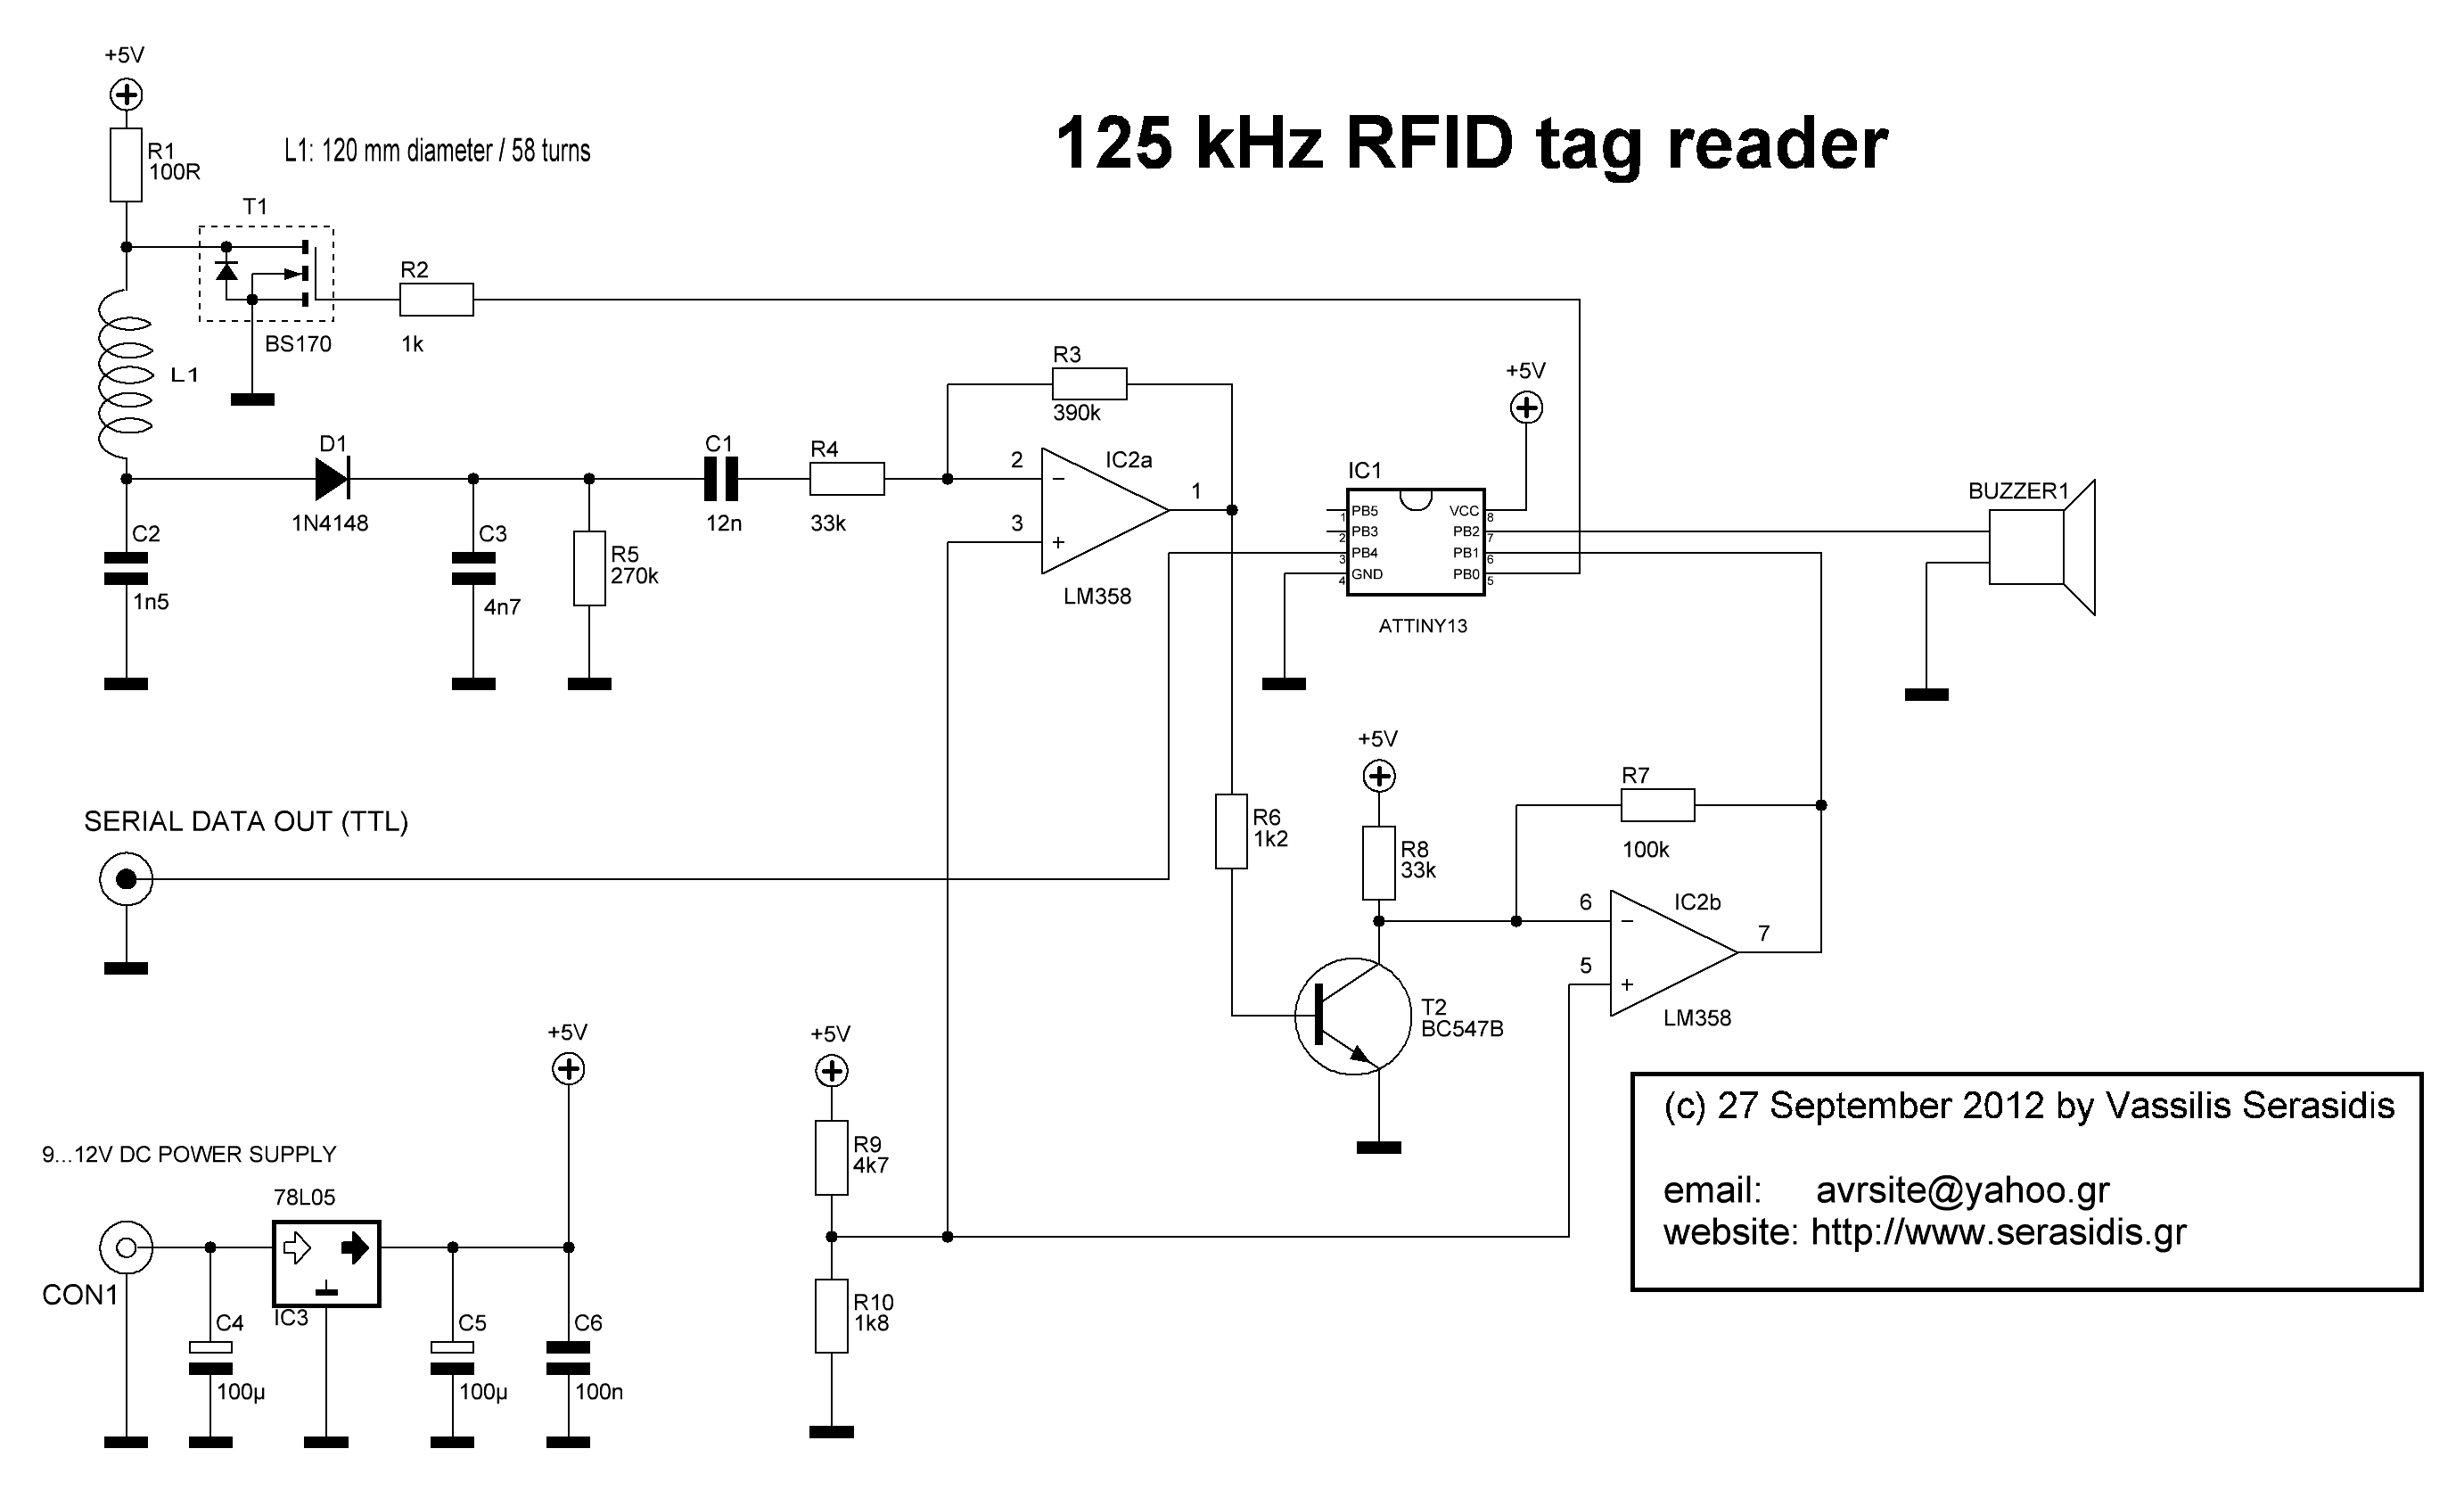
\includegraphics[width=1.5\textwidth]{02_Literature_study/figures/125kHz_RFID_reader_schem.png}
  \caption{Circuit diagram for Vassilis Serasidis solution}
  \label{fig:02:ATtiny13Circuit}
 \end{figure}
\end{landscape}

\newpage

\subsection{Potential threats and vulnerabilities}
There are numerous ways to intercept and or attack RFID systems. Several of these attacks can be hard to defend against. The reason being that some are near undetectable, while some only seek to disable the system, either temporarily or permanently. Some of the ways to attack an RFID system include:

\begin{labeling}{EMP tag destruction}
    \item[Skimming] By eavesdropping while transmission is occurring, if one knows the air protocol used it is possible to retrieve the tag's data without actively interfering with the system.
    
    \item[EMP tag destruction] An attacker sets of an electromagnetic pulse frying the antenna and chip of the RFID system. This is a pure physical attack and serves no other purpose than to hinder the use of the system.
    
    \item[Cloning] A cloning attack might be the most famous of RFID weaknesses. The fact that the tags on 125kHz in particular has few to none security measures, it is possible to copy the tag ID into ones own tag. This could grant access to whatever the original tag opens, or identifying itself as the original tag. This is why a PIN code is usually used in conjunction with such access cards.
    
    \item[Jamming] During a jamming attack, the attacker sends out a high effect radio signal with random data in the frequency range the RFID system is running on. This will make it impossible to read any tag while the attack is occuring.
    
    \item[Location] Here one is not so much interested in \textit{what} the ID is as the \textit{where} the tag is located. This type of attack works even if the data sent by the tag in encrypted. By associating a tags encrypted hash, The attacker would be able to know where it is used, even without knowing the actual data of the tag. 
    
    \item[DoS] Denial of service attack in RFID is done by simulating an infinite amount of tags within the range of a reader. Even if the reader has some form of anti-collision mechanism, it will simply be overwhelmed.
    
    \item[Input Validation] As is the case for most network and back-end systems, an attacker might find it possible to inject malicious or false tags into the system by using a rouge reader. This would somewhat be an equivalent to an SQL injection.
    
    \item[Replay] Here the attacker seeks to recreate a session between a tag and a reader to gain access by reenact the session.
\end{labeling}

\subsubsection{Prevention and countermeasures}

The vast majority of attacks on RFID systems depend on the attacker being in close proximity to a reader/access point. So by being aware of where such readers are located and making sure that a PIN is required where there is human-machine interaction, like building access, most attacks can be prevented.

\subsubsection{Concerns}


Stop RFID is an anti-RFID movement that opposes the use of RFID in consumer products for privacy concerns. With RFID they argue that there are two main concerns:


\begin{enumerate}
    \item If an RFID tag is implemented onto consumer products, the tag might be read by anyone without the purchasers knowledge or approval. Behavioral patterns and purchases are considered sensitive information that should not be public or easily obtainable.
    \item In the event that an RFID tagged product is purchased using a credit card or a in conjunction with a loyalty card, it would be possible to deduce who purchased the item if in possession of either the credit card information or the loyalty card.
\end{enumerate}

For the most part, these problems can be counteracted by limiting the reading distance of the tags. This would make it near impossible for a victim not to know that someone was scanning their products. The second concern is an unlikely event as something physical would have to be stolen first, either the credit card or the loyalty card.

